\documentclass{standalone}

\usepackage[OT1]{fontenc}
\renewcommand*\familydefault{\sfdefault}
\usepackage{helvet,sfmath}
\usepackage{siunitx}

\usepackage{tikz}
\usepackage{circuitikz}

\definecolor{BlueDefault}{rgb}{0.2,0.2,0.7}

\begin{document}

\begin{circuitikz}[scale=0.6]
    %% Transmission line
    \foreach \x in {-9,0,9}
    \draw
    ( \x + 0,0) to[short, o-o] ( \x + 9,0)
    ( \x + 0,3) to[inductor, l=\(L\), o-] ( \x + 2.5,3) to[generic, l=\(R\)] ( \x + 5,3) to[short, -o] ( \x + 9,3)
    ( \x + 5.5,3) to[capacitor, l=\(C\)] ( \x + 5.5,0)
    ( \x + 7.5,3) to[generic, l=\(G\)] ( \x + 7.5,0)
    ;
    \draw[BlueDefault, thick, dashed] (0,-1) to (0,4.5) to (9,4.5) to (9,-1) to (0,-1);
    \draw[Stealth-Stealth] (0,5) to (9,5);
    \draw (4.5,5) node[above]{\(\Delta x\)};
    %% YZ model
    \draw 
    (10.5,-5) to[short, o-o] (16.5,-5)
    (10.5,-2) to[short, o-] (11.5,-2) to[generic, l=\(Z\)] (14,-2) to[short, -o] (16.5,-2)
    (15,-2) to[generic, l=\(Y\)] (15,-5)
    ;
    \draw[BlueDefault, thick, dashed] (10,-5.5) to (17,-5.5) to (17,-0.5) to (10,-0.5) to (10,-5.5);
    \draw[BlueDefault, thick, dashed] 
    (0,-1) to (10,-5.5)
    (9,4.5) to (17,-0.5)
    ;
    %% Node
    \draw
    (-4,10) node{ \Large \( \lim_{\Delta x \rightarrow 0} \frac{Y}{\Delta x} = j \omega \varepsilon_{eff}, \)}
    (-4,8) node{ \Large \( \lim_{\Delta x \rightarrow 0} \frac{Z}{\Delta x} = j \omega \mu_{eff}. \)}
    (-4,-2) node{ \Large \( n = \sqrt{\mu_{eff} \varepsilon_{eff} } \)}
    (-4,-4) node{ \Large \( Z_B = \sqrt{\frac{\mu_{eff}}{\varepsilon_{eff}}}\)}
    ;
    \draw[BlueDefault, thick, -Stealth] (-5.5,4.5) to (-2.5,4.5);
    \draw (-4,4.5) node[above]{Wave};
    \draw[BlueDefault, thick, -Stealth] (14,-2.5) to (14,-4.6);
    \draw (13.5,-3.6) node{\(\mathbf{E}\)};
    \draw[BlueDefault, thick] (11.9,-3.6) circle (0.3);
    \draw[BlueDefault, fill=BlueDefault, thick] 
    (11.8,-3.5) to (12.0,-3.7)
    (11.8,-3.7) to (12.0,-3.5)
    ;
    \draw (11.3,-3.6) node{\(\mathbf{H}\)};

    \draw (11.5,8.5) node{ 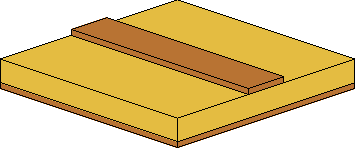
\includegraphics[width=200pt]{Figures/Microstrip_line.pdf} };
\end{circuitikz}

\end{document}

